%% -*- coding: utf-8 -*-
\documentclass[12pt,a4paper]{scrartcl} 
\usepackage[utf8]{inputenc}
\usepackage[english,russian]{babel}
\usepackage{indentfirst}
\usepackage{misccorr}
\usepackage{graphicx}
\usepackage{amsmath}
\begin{document}
\section{Введение}
\label{sec:intro}

% Что должно быть во введении
\begin{enumerate}
 \item Текстовая формулировка задачи
 \item Пример кода, решающего данную задачу
 \item Скриншот программы
\end{enumerate}
\section{Ход работы}
\label{sec:exp}
\subsection{Код приложения}
\label{sec:exp:code}
\begin{verbatim}
Генератор случайных чисел Парка-Миллера с перетасовкой
#include <stdio.h>
#define IA 16807
#define IM 2147483647
#define AM (1./IM)
#define IQ 12773
#define IR 2836
#define NTAB 32
#define NWUP 8
#define NDIV (1+(IM-1)/NTAB)
#define EPS 1.2e-7
#define RNMX (1.0-EPS)
#define MASK 123456789

static long dummy;
void Seed(long dum) {
	dummy = dum;
}

float unirand0(void) {
	long k;
	float ans;

	dummy ^= MASK;	
	k = dummy / IQ;

	if ((dummy = IA * (dummy - k * IQ) - IR * k) < 0)
		dummy += IM;

	ans = AM * dummy;

	dummy ^= MASK;	

	return(ans);
}

float unirand1(void) {
	int j;
	long k;
	static long iy = 0, iv[NTAB];
	float temp;
	
	if (dummy <= 0 || !iy) {
		if (dummy < 0) dummy = -dummy; else
			if (dummy == 0) dummy = 1;
		for (j = NTAB + NWUP - 1; j >= 0; j--) {
			k = dummy / IQ;

			if ((dummy = IA * (dummy - k * IQ) - IR * k) < 0)
				dummy += IM;

			if (j < NTAB)
				iv[j] = dummy;
		}

		iy = iv[0];
	}

	k = dummy / IQ;
	if ((dummy = IA * (dummy - k * IQ) - IR * k) < 0)
		dummy += IM;

	iy = iv[j = iy / NDIV];
	iv[j] = dummy;

	if ((temp = AM * iy) > RNMX)
		return(RNMX);
	else
		return(temp);
}

int main() {
	int i;
	Seed(6723);
	for (i = 0; i < 100; i++)
		printf("%f\n", unirand1());
}

Генератор случайных чисел Парка-Миллера без перетасовки
#include <stdio.h>
#define IA 16807
#define IM 2147483647
#define AM (1./IM)
#define IQ 12773
#define IR 2836
#define MASK 123456789

static long dummy;
void Seed(long dum) {
	dummy = dum;
}

float unirand0(void) {
	long k;
	float ans;

	dummy ^= MASK;
	k = dummy / IQ;

	if ((dummy = IA * (dummy - k * IQ) - IR * k) < 0)
		dummy += IM;

	ans = AM * dummy;

	dummy ^= MASK;

	return(ans);
}

int main() {
	int i;
	Seed(6723);
	for (i = 0; i < 100; i++)
		printf("%f\n", unirand0());
}
\end{verbatim}
\subsection{формулы}
\label{sec:mathexample}

Общая формула генератора случайных чисел \ Xk+1=a * Xk  mod m
\newpage
\begin{document}
\section{Пример скриньшота программы }
Генератор случайных чисел Парка-Миллера с перетасовкой
\label{sec:picexample}
\begin{figure}[h]
\centering
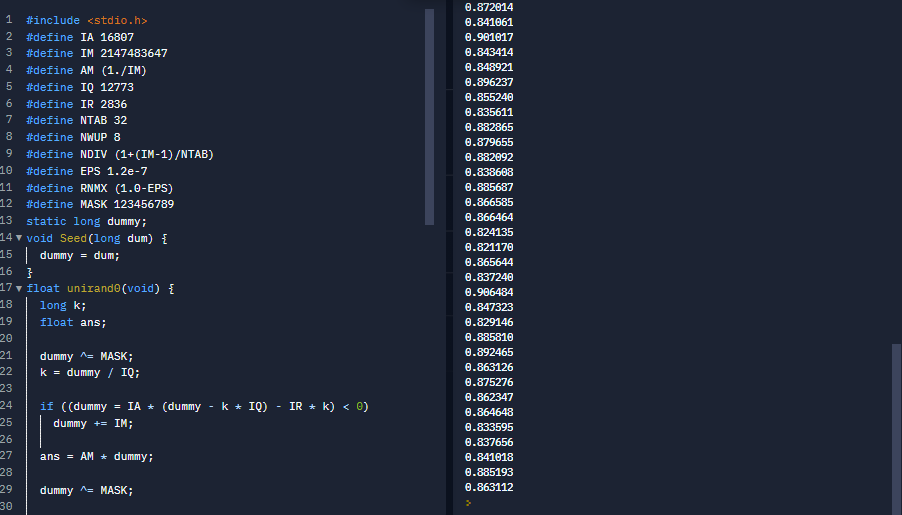
\includegraphics[scale=0.5]{скрин по с++.png}
\caption{скриньшот программы}\label{fig:par}

\end{figure}
\newpage
\begin{document}
\label{sec:picexample}
\begin{figure}[h]
\centering
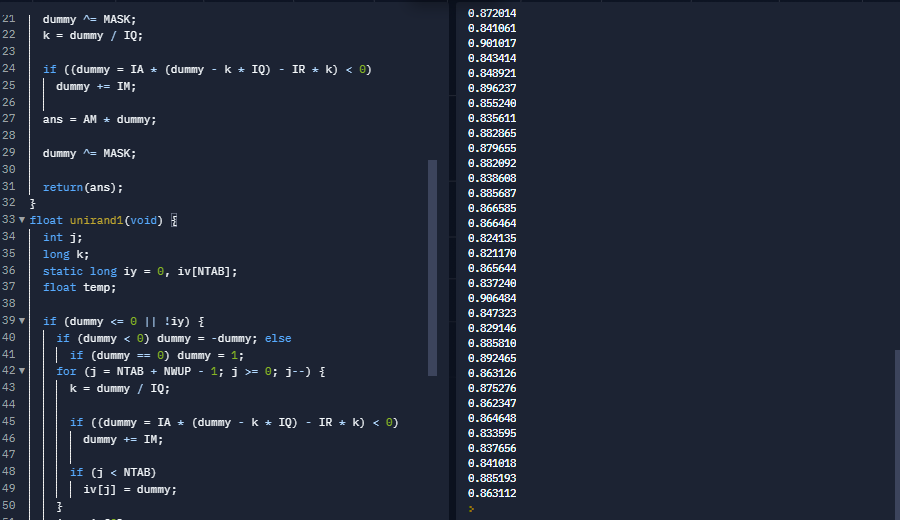
\includegraphics[scale=0.5]{скрин с++ (2).png}
\caption{скриньшот программы}\label{fig:par}

\end{figure}
\newpage
\begin{document}
\label{sec:picexample}
\begin{figure}[h]
\centering
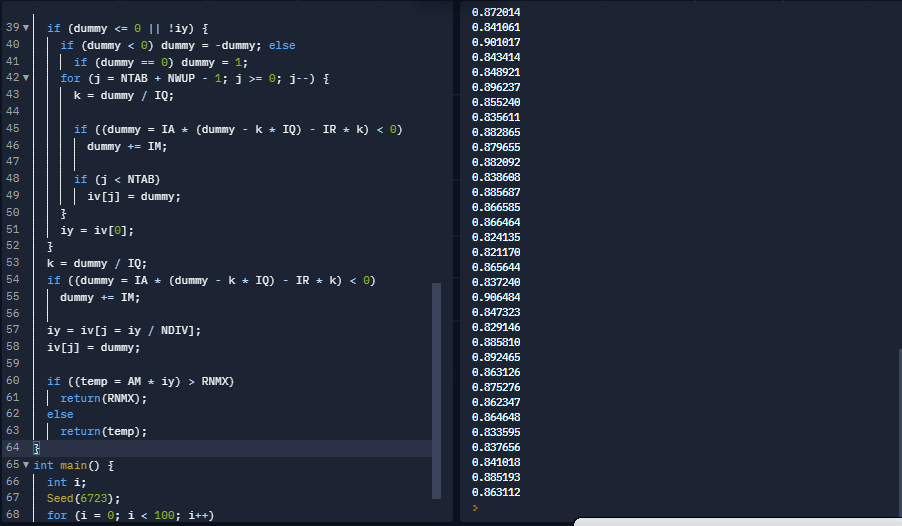
\includegraphics[scale=0.5]{скрин с++ (3).png}
\caption{скриньшот программы}\label{fig:par}
\end{figure}

\newpage
\begin{document}
\label{sec:picexample}
\begin{figure}[h]
\centering
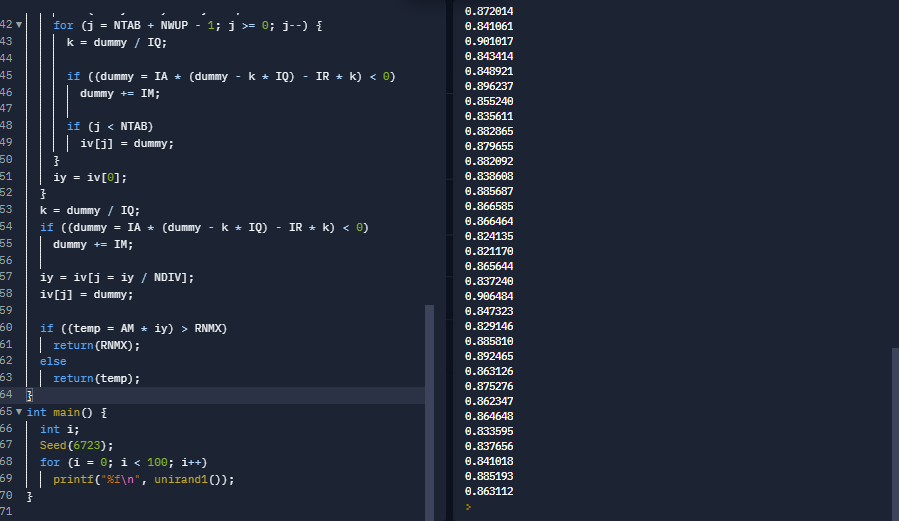
\includegraphics[scale=0.5]{скрин с++ (4).png}
\caption{скриньшот программы}\label{fig:par}
\end{figure}

\newpage
\begin{document}
Генератор случайных чисел Парка-Миллера без перетасовкой
\label{sec:picexample}
\begin{figure}[h]
\centering
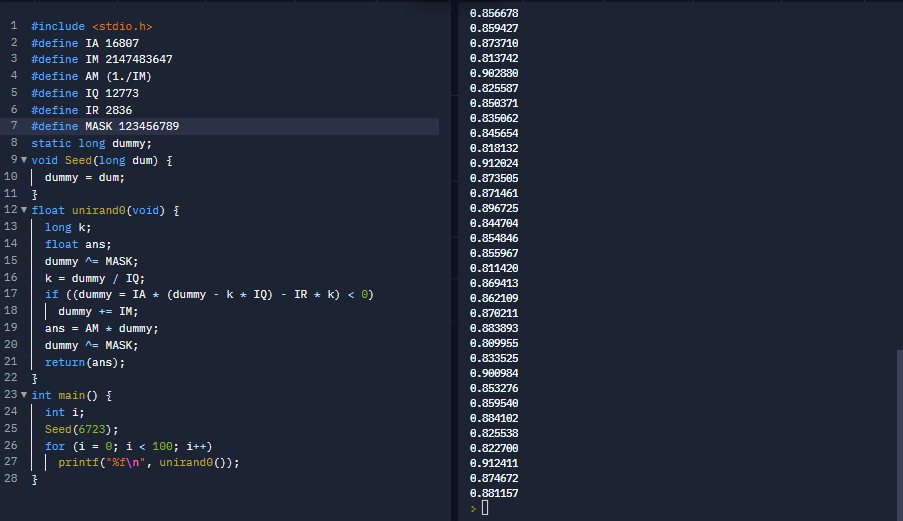
\includegraphics[scale=0.5]{скрин с++ (5).png}
\caption{скриньшот программы}\label{fig:par}
\end{figure}


\section{ библиографические ссылки}

Для изучения «внутренностей» \TeX{} необходимо
изучить~\cite{Knuth-2003}, а для использования \LaTeX{} лучше
почитать~\cite{Lvovsky-2003, Voroncov-2005}.

\begin{thebibliography}{9}
\bibitem{Knuth-2003}Кнут Д.Э. Всё про \TeX. \newblock —- Москва: Изд. Вильямс, 2003 г. 550~с.
\bibitem{Lvovsky-2003}Львовский С.М. Набор и верстка в системе \LaTeX{}. \newblock —- 3-е издание, исправленное и дополненное, 2003 г.
\bibitem{Voroncov-2005}Воронцов К.В. \LaTeX{} в примерах. 2005 г.
\end{thebibliography}
\end{document}
\end{document}
\end{document}